\newpage\part{Flash Cards}

\section{Farmaci del SNC e del SNP}

\begin{tikzpicture}
	\tikzset{level distance=90pt,frontier/.style={distance from root=370pt}} 
	\Tree
	[.SNC
		[.Periferico
			[.Sensitivo ]
			[.Autonomo
		 		[ .{Simpatico\\ (toraco--addominale)} {gangli pre e para--vertebrali} ]
				[ .{Parasimpatico \\(nervi crani e sacrale)} {nell'intima degli organi} ]
			]
			[.Gastroenterico {plessi mioenterici (Auerbach) e\\ sottomucosi (Meissner)}
			]
		]
		[.Centrale ]
	]
\end{tikzpicture}

\begin{tikzpicture}
	\tikzset{level 1/.style={level distance=150pt}}
	\Tree
	[.{Neurotrasmettitori\\ SNP}
		 [.\node(acetilcolina){acetilcolina}; {recettori colinergici} ]
		 [.noradrenalina {recettori adrenergici} ]
		 [.\node(serotonina){serotonina\\5-HT 5-idrossitriptamina}; {recettori serotoninergici} ]
		 [.{monossido d'azoto (NO)} ] 
		 [.purine ]
	]
	\begin{scope}[yshift=-9em]
	\Tree
	[.\node(snc){Neurotrasmettitori\\ SNC};
		[.dopamina {recettori dopaminergici} ]
		Glutammato
		GABA
	]
	\end{scope}
	\draw[drawarrow] (snc.east) to[in=180,out=40] (acetilcolina.west)
		(snc.east) to[in=180,out=0] (serotonina.west);
\end{tikzpicture}

\subsection{Acetilcolina}

\begin{tikzpicture}
	\tikzset{level 1/.style={level distance=150pt}}
	\Tree
	[.localizzazione {tutte le fibre pregangliali sia para che orto\\ nicotiniche} {parasimpatiche post gangliali (quasi tutte).\\ muscariniche} {ghiandole sudoripare (simpatico)\\ muscariniche} {giunzione neuromuscolare\\ nicotiniche} ]
\end{tikzpicture}

\begin{tikzpicture}
	\tikzset{level 2/.style={level distance=130pt}, level 3/.style={level distance=120pt}}
	\Tree
	[.Sintesi
		[.colina \edge node[smallfont,yshift=5pt,xshift=5.4em]{entra nel neurone} node[smallfont,yshift=-5pt,xshift=5.4em]{tappa limitante};
			[.{acetilCOA + colina} \edge node[smallfont,yshift=-5pt,xshift=5em]{acetiltrasferasi} node[smallfont,yshift=5pt,xshift=5em]{colina}; acetilcolina ]
		]
	]
\end{tikzpicture}

\begin{tikzpicture}
	\tikzset{level 2/.style={level distance=130pt}}
	\Tree
	[.Degradazione
		[.acetilcolina \edge node[smallfont, yshift=-5pt,xshift=5.5em]{acetilcolinesterasi}; {acetato + colina} ]
	]
\end{tikzpicture}

\begin{tikzpicture}
	\Tree
	[.Liberazione 
		[.{Ca${}^{2+}$ + VAMP/SNAPS}
			[.{fusione vescicole con\\ membrana neuronale} esocitosi
			]
		]
	]
\end{tikzpicture}

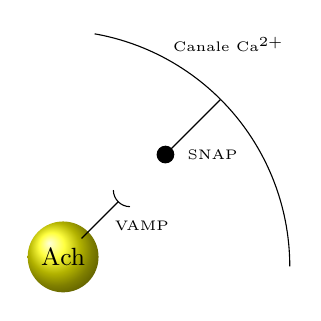
\begin{tikzpicture}
	\tikzstyle{cwhite}=[circle,shadedraw=yellow];
	\shade[ball color=yellow] node (ach) {\small Ach} circle[radius=.45];
	\draw (ach) -- +(.7,.7) +(.7,.7) arc [start angle=225, end angle=270, radius=6pt]  (.7,.7) arc [start angle=225, end angle=180, radius=6pt];
	\draw (2,2) arc [start angle=45, end angle=0, radius=3cm];
	\draw (2,2) arc [start angle=45, end angle=80, radius=3cm];
	\draw (2,2) -- (1.3,1.3);
	\filldraw (1.3,1.3) circle[radius=3pt];
	\node at (1,.4) {\tiny VAMP};
	\node at (1.9,1.3) {\tiny SNAP};
	\node at (2.1,2.7) {\tiny Canale Ca${}^{2+}$};
\end{tikzpicture}

\begin{tikzpicture}
	\Tree
	[.Effetti
		[.{$\uparrow$permeabilit\`a ai cationi\\ Na${}^+$, K${}^+$, Ca${}^{2+}$}
			[.depolarizzazione
				[.{fibre post sinaptiche} PdA ]
				[.{fibre muscolari} {generazione potenziale\\ di placca}
				]
			]
		]
	]
\end{tikzpicture}

\begin{tikzpicture}
	\tikzset{level 1/.style={level distance=80pt},level 2/.style={level distance=140pt},level 3/.style={level distance=140pt}}
	\Tree
	[.{Recettore colinergico}
		[.{muscarinico\\ (metabotropo)}
			[.{M${}_1$ eccitatorio $\uparrow\text{IP}_3, \uparrow\text{DAG},\uparrow\text{Ca}^{2+}$} {SNC, simpatico post--gangliare,\\ cellule parietali dello stomaco}
			]
			[.{M${}_2$ inibitorio $\downarrow$cAMP } {cuore, muscolo liscio}
			]
			[.{M${}_3$ eccitatorio $\uparrow\text{IP}_3, \uparrow\text{DAG},\uparrow\text{Ca}^{2+}$} {ghiandole esocrine, muscolo liscio,\\ endotelio dei vasi}
			]
			[.{M${}_4$ come $\text{M}_2$} {SNC}
			]
			[.{M${}_5$  come $\text{M}_1$} {endotelio vasale, cervello, SNC}
			]
		]
		[.{nicotinico\\ (ionotropo)}
			[.{N${}_\text{N}$ gangliare} {para e ortosimpatico gangliare} ]
			[.{N${}_\text{M}$ muscolare} {giunzione\\ neuromuscolare} ]
		]
	]
\end{tikzpicture}

\subsubsection{Agonisti colinergici}

\begin{tikzpicture}
	\tikzset{
		level distance=80pt,
		level 1/.style={level distance=70pt},
		level 2/.style={level distance=70pt},
		frontier/.style={distance from root=400pt} 
	}
	\Tree
	[.\node(main){Tipo}; 
		[.diretti
			[.{attivano recettori} 
				[.{esteri della colina} 
					\node(ach){acetilcolina };
					metacolina
					carbacolo
					\node[farmaco](beta){betanecolo};
				]
				[.alcaloidi
					[.muscarinici
						muscarina
						\node[farmaco]{pilocarpina};
					]
					[.nitotinici \node[farmaco]{nicotina}; ]				
				]
			]
		]
		[.indiretti
			[.\node(AchEI){inibitori AchE}; 
				\node[farmaco](neo){neostigmina};
				\node[farmaco]{edrifonio}; 
				[.{organofosfati} \node[farmaco]{ecotiopato}; ]
				\node(somar){somar (gas nervino)};  
			]
		]
	]	
	\node[right=5pt of somar] (somary) {};
	\node[above=6em of somary] (neox) {};
	\draw[drawarrow] (neox) -- (somary) node[midway,above,sloped] {\tiny $\uparrow$durata azione};
	\node[right=5pt of ach] (achn) {};
	\node[right=5pt of beta] (betan) {};
	\draw[drawarrow] (achn) -- (betan) node[midway,above,sloped] {\tiny $\uparrow$resist. idrolisi e quindi durata azione};
\end{tikzpicture}

\begin{tikzpicture}
	\Tree
	[.{Inibitori AchE}
		[.{alcool+gruppo N quaternario}
			[.\node[farmaco]{edrofonio}; 
				[.{legame idrogeno\\ o ionico con AchE} {idrolisi in minuti}
				]
			]
		]
		[.carbammati 
			[.\node[farmaco]{neostigmina\\ fisostigmina}; 
				[.{legame covalente con AchE} {idrolisi in ore}
				]
			]
		]
		[.organofosfati
			[.somar
				[.\node(fAchE){fosforilazione AchE}; \node(idro){idrolisi in giorni};
				]
			]
			\node[farmaco](ecotiopato){ecotipato};
		]
	]		
	\draw[drawarrow] (ecotiopato) to[out=0,in=180] (fAchE);
	\node[chartnode,below=1em of fAchE] (invec) {invecchiamento\\rottura legame O-P\\ con raffozamento\\ legame con AchE}; 
	\node[chartnode,below=1em of idro] (pral) {pralidossina pu\`o\\ scindere la\\ fosforilazione};
	\draw[drawarrow] (pral)--(fAchE) node[midway,above,sloped] {\tiny qui si};
	\draw[drawarrow] (pral)--(invec) node[midway,above,sloped] {\tiny qui no};
\end{tikzpicture}

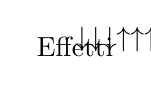
\begin{tikzpicture}
	\tikzset{level distance=120pt, level 2/.style={level distance=150pt}}
	\Tree
	[.\node(sub){Effetti}; 
		[.occhio 
			{contrazione muscolo sfintere dell'iride (miosi)\\ contrazione muscolo ciliare (accomodamento da vicino)}
		]
		[.cuore
			{$\downarrow$frequenza (cronotopo-), $\downarrow$forza (inotropo-),\\ $\downarrow$vel. conduzione (dromotropo-), $\uparrow$periodo refrattario, NAV}
		]
		[.vasi
			{dilatazione a basse dosi o contrazione a alte dosi}
		]
		[.polmone
			 {broncocostrizione, $\uparrow$secrezione}
		]
		[.intestino
			{$\uparrow$motilit\`a, $\downarrow$ muscolatura sfinteri, $\uparrow$ secrezioni} 
		]
		[.vescica
			 {contrazione destrusore, rilascio trigono}
		]
		[.{ghiandole sudoripare\\ lacrimali\\ salivali} 
			{$\uparrow$secrezioni}
		]
		[.{giunzione neuromuscolare\\ (indiretti)}
			{basse concentrazioni: $\uparrow$forza contrazione utile \\ se intossicazioni da curaro o miastenia grave\\ alte concentrazioni: fibrillazione fibre muscolari}
		]
	]
\end{tikzpicture}

\begin{tikzpicture}
	\tikzset{level distance=130pt, level 2/.style={level distance=160pt},frontier/.style={distance from root=300pt}}
	\Tree
	[.{usi clinici\\ agonisti colinergici}
		[.occhio {glaucoma con diminuzione della pressione\\ nelle emergenze ad angolo chiuso,\\ agonista muscarinico (pilocarpina)\\ + inibitore colinesterasi (ecotiopato)\\ 
		nel glaucoma cronico ora si usano i $\beta$-bloccanti.} ]
		[.{gastrointestinale\\ urinari} {Tutti i casi di depressione dell'attivit\`a senza ostruzione\\ neostigmina/betanecolo nelle ritenzioni urinarie e ileo\\
		pilocarpina usata per $\uparrow$secrezioni salivari in xerostomia da\\
		sindrome di Sjogren.} ]
		{intossicazione da\\ farmaci antimuscarinici\\ (intossicazione da atropina)\\ fisostigmina}
		[.cuore {tachiaritmia parossistica sopraventricolare\\ edrofonio(in disuso)\\ ora si usa l'adenosina.} ]
		[.{giunzione neuromuscolare} 
			[.{miastenia grave\\ edofonio/neostigmina} ]
			[.{post anestesia\\ ??? Leggo nelle correzioni\\ NO negli inibitori AchE ma boh!! } ]
		]
	]
\end{tikzpicture}

\subsubsection{Antagonisti colinergici}

\begin{tikzpicture}
	\Tree
	[.{antagonisti\\ colinergici}
		[.antimuscarinici \node[farmaco]{atropina}; \node[farmaco]{scopolamina};
		]
		[.{ganglioplegico\\ antinicotinico} \node[farmaco]{tetraetilammonio (TEA)}; \node[farmaco]{esametanio (C6)};
		]
		[.{rigeneratori dell'AchE} \node[farmaco]{pralidossima\footnotemark};
		]
	]
\end{tikzpicture}

\footnotetext{vedi inibitori dell'AchE}

\begin{tikzpicture}
	\tikzset{level 2/.style={level distance=160pt}}
	\Tree
	[.{anti-muscarinici\\ effetti}
		[.SNC {effetto stimolante (-atropina +scopolamina) $\downarrow$ tremore parkinson}
		]
		[.occhio {$\uparrow$attività simpatica $\Rightarrow$ midriasi\\ (belladonna $\equiv$ occhi dilatati)}
		]
		[.cuore {tachicardia, blocco vagale, $\downarrow$PR per $\uparrow$dromotropo}
		]
		[.vasi incerta ]
		[.{apparato respiratorio} {broncodilatazione, $\downarrow$secrezioni\\ (ma meglio i $\beta$-adrenergici)}
		]
		[.{gastrointestinale} {$\downarrow$secrezioni salivali, minori su tutto il resto} ]
		[.{gh. sudoripare} {soppressione termoregolazione\\ (febbre da atropina)} ]
	]
\end{tikzpicture}

\begin{tikzpicture}
	\tikzset{level 1/.style={level distance=130pt}}
	\Tree
	[.{anti-muscarinici\\ usi clinici} 
		{malattia di Parkinson} 
		{chinetosi} 
		{occhio} 
		{apparato respiratorio} 
		{apparato cardiovascolare} 
		{apparato gastrointestinale} 
		{apparato urinario}
	]
\end{tikzpicture}

\begin{tikzpicture}
	\Tree
	[.{rigeneratori\\ dell'AchE}
	]
\end{tikzpicture}

\subsection{Noradrenalina}

\begin{tikzpicture}
	\Tree
	[.noradrenalina 
		[.{simpatiche postgangliari} 
			[.escluso
				{muscolatura vasi renali ($\text D_1$)}
				{ghiandole sudoripare (Ach)}
			]
		]		
	]
\end{tikzpicture}

\begin{tikzpicture}
	\begin{scope}
	\tikzset{level distance=90pt,level 3/.style={level distance=150pt},
	level 2/.style={level distance=130pt},level 4/.style={level distance=60pt}}
	\Tree 
	[.Sintesi 
		[.Tirosina  \edge node[smallfont,yshift=-5pt,xshift=5.5em]{tirosin--idrossilasi} node[smallfont,yshift=5pt,xshift=5.5em]{tappa limitante}; 
			[.{L-Dopa} \edge node[smallfont,yshift=-5pt,xshift=6em]{DOPA decarbossilasi};
				[.\node[farmaco]{dopamina}; \node[dummyc]{};]
			]
		]
	]
	\end{scope}
	\begin{scope}[yshift=-3em,xshift=1em]
	\tikzset{level distance=80pt}
	\Tree
	[.\node[dummyc]{}; 
		[.\node[farmaco]{noradrenalina}; \node[farmaco]{adrenalina};]
	]	
	\end{scope}				
	
\end{tikzpicture}

\begin{tikzpicture}
	\tikzset{level distance=130pt}
	\Tree 
	[.Degradazione
		[.{MAO (mono-ammino ossidasi)\\ in fegato e cellule ?????} ]
		[.{COMT (catecolo O-metiltransferasi)\\ nei neuroni} ]
	]
\end{tikzpicture}

\begin{tikzpicture}
	\tikzset{level 2/.style={level distance=150pt}}
	\Tree	
	[.{Recettore adrenergico\\ (metabotropo \\ a proteine G)} 
		[.{$\alpha$}
			[ .{$\alpha_1\,\text{G}_{\text{q}} \uparrow\text{IP}_3, \uparrow\text{Ca}^{2+}$ (postsinaptiche muscolo liscio)} ]
			[ .{$\alpha_2\,\text{G}_{\text{i}} \downarrow\text{cAMP}$ (presinaptiche muscolo liscio)} ]
		]
		[.{$\beta$}
			[.{$\beta_1\,\text{G}_{\text{s}} \uparrow\text{cAMP}$ (postsinaptiche cuore, adipociti,\\ iuxaglomerulare, epitelio corpi ciliari)} ]
			[.{$\beta_2\,\text{G}_{\text{s}} \uparrow\text{cAMP}$ (postsinaptiche muscolo liscio e cuore)} ]
			[.{$\beta_3\,\text{G}_{\text{s}} \uparrow\text{cAMP}$ (postsinaptiche cuore, adipociti, vescica)} ]		
		]
	]
\end{tikzpicture}

\begin{tabular}{|c|c|c|c|}
\hline 
\textbf{Organo} & \textbf{Tipo} & \textbf{Recettore} & \textbf{Azione} \\ 
\hline\hline 
M. radiale & simpatico & $\alpha_1$ & costrizione \\ 
\hline 
M. circolare & parasimpatico & M${}_3$ & costrizione pupilla \\ 
\hline 
M. ciliare & simpatico & $\beta$ & rilasciamento \\ 
\hline 
M. ciliare & parasimpatico & M${}_2$ & contrazione \\ 
\hline 
Nodo SA & simpatico & $\beta_1\beta_2$ & accellerazione \\ 
\hline 
Nodo SA & parasimpatico & M${}_2$ & rallentamento \\ 
\hline 
Forza contrazione & simpatico & $\beta_1\beta_2$ & aumento \\ 
\hline 
Forza contrazione & parasimpatico & M${}_2$ & diminuzione \\ 
\hline 
vasi muscolari & simpatico & $\beta$ & rilasciamento \\ 
\hline 
muscolo gastrointestinale & simpatico & $\alpha_2\beta_2$ & rilasciamento \\ 
\hline 
muscolo gastrointestinale & parasimpatico & M${}_3$ & contrazione \\ 
\hline 
sfinteri gastrointestinali & simpatico & $\alpha_1$ & contrazione \\ 
\hline 
sfinteri gastrointestinali & parasimpatico & M${}_3$ & rilasciamento \\ 
\hline 
\end{tabular} 

\subsection{Serotonina}

Serotonina o 5-HT o 5-idrossitriptamina

\begin{tikzpicture}
	\tikzset{level 3/.style={level distance=130pt}}
	\Tree
 	[.Recettore
 		[.5-HT1
 			[.SNC {GpCR,$\downarrow$cAMP, inibizione presinaptica} ]
 		]
 		[.5-HT2
 			[.{muscolo liscio\\ piastrine} {$\uparrow$IP3, DAG, GpCR} ]
 		]
 		[.5-HT3
 			[.{SNP (nocicettori\\ neuroni enterici)} {canale ionico stimolatore} ]
 		]
 		[.5-HT4
 			[.{SNC,vescica\\ cuore} {$\uparrow$cAMP,GpCR,eccitazione} ]
 		]
 	]
\end{tikzpicture}

\begin{tikzpicture}
	\tikzset{level distance=80pt,level 3/.style={level distance=130pt},
	level 2/.style={level distance=130pt}}
	\Tree 
	[.Sintesi 
		[.Triptofano  \edge node[smallfont,yshift=5pt,xshift=5.5em]{triptofano} node[smallfont,yshift=-5pt,xshift=5.5em]{idrossilasi} ; 
			[.{5-idrossitriptofano} \edge node[smallfont,yshift=5pt,xshift=5.5em]{amminoacido} node[smallfont,yshift=-5pt,xshift=5.5em]{decarbossilasi}; 5-HT 
			]
		]
	]	
\end{tikzpicture}

\begin{tikzpicture}
	\tikzset{level distance=130pt}
	\Tree 
	[.Degradazione {MAO (mono-ammino ossidasi)}
	]
\end{tikzpicture}

\begin{tikzpicture}
	\tikzset{level distance=160pt}
	\Tree
	[.Effetti {piastrine: aggregazione} {terminazioni nervose: dolore} {SNC: eccitatorio 5-HT4,\\ inibitorio 5-HT1} {vasi: costrizione} {gastroenterico: attivazione secrezione\\ e peristalsi} ]
\end{tikzpicture}

\subsection{Neurotrasmettitori purinici}

\begin{tikzpicture}
	\tikzset{level 2/.style={level distance=130pt}}
 	\Tree
 	[.{Neurotrasmettitori\\ purinici} 
 		[.ATP {Aumento della permeabilit\`a di membrana} ]
 		[.Adenosina {vasodilatatore tranne che nel rene} {inibizione dell'aggreg. piastrinica} {blocco della conduzione AV}
 		]
 	]
\end{tikzpicture}

\subsection{Monossido d'azoto (NO)}

\begin{tikzpicture}
	\Tree
	[.Tipi
		[.iNOS {prodotto dai macrofagi tramite IF$\gamma$}
		]
		[.eNOS {endotelio e piastrine}
		]
		[.nNOS neuroni
		]
	]
\end{tikzpicture}

\begin{tikzpicture}
	\tikzset{level distance=160pt}
	\Tree
	[.Causa {vasodilatazione} {inibizione dell'aggregazione piastrinica} {plasticit\`a sinaptica} {difesa da cellule neoplastiche, batteri, parassiti} ]
\end{tikzpicture}

Per via inalatoria $\downarrow$shunt, $\downarrow$broncocostrizione, $\downarrow$ipertensione polmonare e quindi utile anche nella cura dell'asma.

Utile nel trattamento delle malattie neurovegetative e shock settico dove aumenta e nell'ateorscelosi e ipercolesterolemia dove diminuisce. 

\subsection{Dopamina}

\begin{tikzpicture}
	\tikzset{level distance=130pt}
	\Tree
	[.{Recettore dopaminergico}
		[.{$\text D_1$, $\text D_5$, eccitatorio, $\uparrow$cAMP} {cervello, muscolatura vasi rene} 
		]
		[.{$\text D_2$, inibitorio, apertura canali $\text K^+$} {cervello, muscolatura liscia} 
		]
		[.{$\text D_3$, inibitorio, apertura canali $\text K^+$} {cervello} 
		]
		[.{$\text D_4$, inibitorio, apertura canali $\text K^+$} {cervello, sistema cardio vascolare} 
		]
	]
\end{tikzpicture}

\newpage